\documentclass{beamer}
\usepackage[utf8]{inputenc}
\usepackage[T1]{fontenc}
\usepackage{fourier}
\usepackage{amssymb}
\usepackage{listings}
\usepackage{graphicx}
\usepackage{clrscode3e}
\usepackage{braket}
\lstset{language=Java,
        basicstyle=\ttfamily\small,
        keywordstyle=\color{blue},
        commentstyle=\color{olive}}
\renewcommand{\emptyset}{\varnothing}
\title{Il cubo di Rubik (e come risolverlo)}
\author[S.~Angeleri, A.~Menti, M.~Zago]{Stefano Angeleri, Alessandro Menti,
Mattia Zago}
\date{}
\setbeamertemplate{navigation symbols}{}
\begin{document}
\begin{frame}
\maketitle
\end{frame}

\begin{frame}
\frametitle{Alcune definizioni}
\begin{columns}
\begin{column}{.45\textwidth}
\begin{itemize}
\item<1,2,3,4,5,6> Considereremo un cubo $3\times 3$
\item Ogni faccia (\emph{side}) ha un colore standard a essa associato (vedi
figura)
\item Ognuno dei nove pezzi di ogni faccia è detto \emph{facelet}
\item Il cubo ha $3$ colonne/righe (\emph{columns}/\emph{rows}), $3$ colonne
laterali (\emph{lateral columns}), $4$ angoli (\emph{corners}) e $8$ spigoli
(\emph{edges})
\end{itemize}
\end{column}
\begin{column}{.45\textwidth}
\centering
\only<1>{\includegraphics[width=\textwidth,keepaspectratio]{%
RubikCubeFaint.png}

\phantom{Cg}}
\pause
\only<2>{\includegraphics[width=\textwidth,keepaspectratio]{%
RubikCubeColumn.png}

Colonna}
\pause
\only<3>{\includegraphics[width=\textwidth,keepaspectratio]{%
RubikCubeRow.png}

Riga}
\pause
\only<4>{\includegraphics[width=\textwidth,keepaspectratio]{%
RubikCubeLateralColumn.png}

Colonna laterale}
\pause
\only<5>{\includegraphics[width=\textwidth,keepaspectratio]{%
RubikCubeCorners.png}

Angolo}
\pause
\only<6>{\includegraphics[width=\textwidth,keepaspectratio]{%
RubikCubeEdges.png}

Spigolo}
\end{column}
\end{columns}
\end{frame}

\begin{frame}
\frametitle{Il problema}
Riarrangia il cubo (ruotando righe, colonne e/o colonne laterali) finché tutte
le facelet su ogni faccia non hanno lo stesso colore.
\end{frame}

\begin{frame}
\frametitle{Notazione di Singmaster}
\begin{itemize}
\item Ogni faccia è descritta da una lettera: \textbf{F} (Front), \textbf{B}
(Back), \textbf{U} (Up), \textbf{D} (Down), \textbf{L} (Left), \textbf{R}
(Right)
\item Ogni mossa può essere vista come una rotazione di un quarto di giro di
una faccia in senso orario (N.B.: si assume che il solutore abbia la faccia di
fronte a sé): \textbf{U} = ruota la faccia ``Up'' di un quarto di giro in senso
orario
\item Il simbolo $'$ indica una rotazione in senso antiorario
\item Le rotazioni di righe/colonne/colonne laterali centrali sono denotate da
\textbf{M} (\emph{middle} --- livello fra L e R), \textbf{E} (\emph{equator}
--- livello fra U e D), \textbf{S} (\emph{standing} --- livello fra F e B)
\item Per denotare le rotazioni del cubo si usano altre lettere: \textbf{X}
(rotazione su R), \textbf{Y} (rotazione su U), \textbf{Z} (rotazione su F)
\end{itemize}
\end{frame}

\begin{frame}
\frametitle{Notazione di Singmaster}
\begin{table}[h]
\begin{tabular}{cccccc}
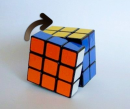
\includegraphics[width=.12\textwidth]{../graphics/moves/F.png} &
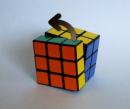
\includegraphics[width=.12\textwidth]{../graphics/moves/F_inv.png} &
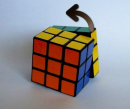
\includegraphics[width=.12\textwidth]{../graphics/moves/B.png} &
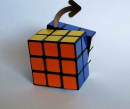
\includegraphics[width=.12\textwidth]{../graphics/moves/B_inv.png} &
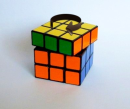
\includegraphics[width=.12\textwidth]{../graphics/moves/U.png} &
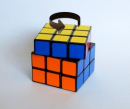
\includegraphics[width=.12\textwidth]{../graphics/moves/U_inv.png} \\
F & F' & B & B' & U & U' \\
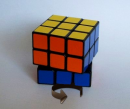
\includegraphics[width=.12\textwidth]{../graphics/moves/D.png} &
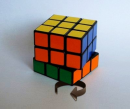
\includegraphics[width=.12\textwidth]{../graphics/moves/D_inv.png} &
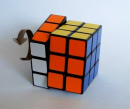
\includegraphics[width=.12\textwidth]{../graphics/moves/L.png} &
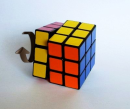
\includegraphics[width=.12\textwidth]{../graphics/moves/L_inv.png} &
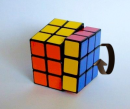
\includegraphics[width=.12\textwidth]{../graphics/moves/R.png} &
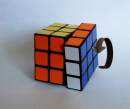
\includegraphics[width=.12\textwidth]{../graphics/moves/R_inv.png} \\
D & D' & L & L' & R & R' \\
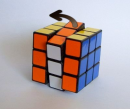
\includegraphics[width=.12\textwidth]{../graphics/moves/M.png} &
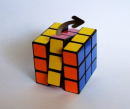
\includegraphics[width=.12\textwidth]{../graphics/moves/M_inv.png} &
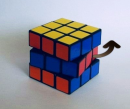
\includegraphics[width=.12\textwidth]{../graphics/moves/E.png} &
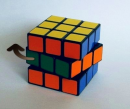
\includegraphics[width=.12\textwidth]{../graphics/moves/E_inv.png} &
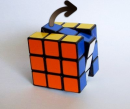
\includegraphics[width=.12\textwidth]{../graphics/moves/S.png} &
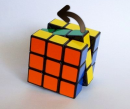
\includegraphics[width=.12\textwidth]{../graphics/moves/S_inv.png} \\
M & M' & E & E' & S & S' \\
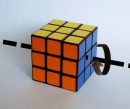
\includegraphics[width=.12\textwidth]{../graphics/moves/X.png} &
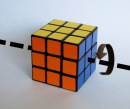
\includegraphics[width=.12\textwidth]{../graphics/moves/X_inv.png} &
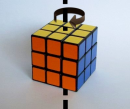
\includegraphics[width=.12\textwidth]{../graphics/moves/Y.png} &
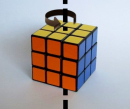
\includegraphics[width=.12\textwidth]{../graphics/moves/Y_inv.png} &
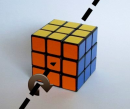
\includegraphics[width=.12\textwidth]{../graphics/moves/Z.png} &
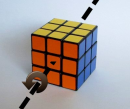
\includegraphics[width=.12\textwidth]{../graphics/moves/Z_inv.png} \\
X & X' & Y & Y' & Z & Z'
\end{tabular}
\end{table}
\end{frame}

\begin{frame}
\frametitle{Il nostro modello}
\begin{itemize}
\item Il cubo è memorizzato in un oggetto \texttt{RubikCubeModel}
\item Ogni faccia è memorizzata in un array $2\times 2$; le righe/colonne sono
numerate dall'alto verso il basso e da sinistra a destra (supponendo che il
solutore abbia la faccia di fronte)
\item \texttt{getSide} determina la faccia che in tale momento ha il colore dato
\item \texttt{getFace} recupera il colore di una facelet
\item Altri metodi autoesplicativi: \texttt{get3DEdge} (per gli angoli),
\texttt{get3DEdgeFacelet} (facelet di un angolo), \texttt{getCorner},
\texttt{getCornerFacelet}
\item Metodi \texttt{rotate*} per ruotare il cubo
\item Test standard: \texttt{isInStandardConfiguration},
\texttt{isWithSaneColors}, \texttt{isSolved}, \texttt{isCornerInPlace},
\texttt{isCornerInPlaceMaybeFlipped}, \texttt{isEdgeInPlace},
\texttt{isEdgeInPlaceMaybeFlipped}
\end{itemize}
\end{frame}

\begin{frame}[fragile]
\frametitle{Mosse di Singmaster}
\begin{itemize}
\item Sono state implementate le mosse standard di Singmaster
\item Ogni mossa (per motivi di astrazione) è una sottoclasse di \texttt{Move}
\item Il costruttore accetta come parametri il modello del cubo (in modo che il
cubo originale rimanga inalterato) e un parametro \texttt{reversed} (per sapere
se la mossa è diretta o inversa)
\item Per applicare una mossa, basta crearla e chiamare
\texttt{perform}/\texttt{reverse}:
\begin{center}
\begin{lstlisting}
(new B(m, reversed)).perform();
\end{lstlisting}
\end{center}
\item Ogni mossa genera un evento per comunicare i cambiamenti all'interfaccia
\end{itemize}
\end{frame}

\begin{frame}
\frametitle{Strategie di risoluzione}
\begin{itemize}
\item Sono sottoclassi di \texttt{ResolutionStrategy}
\item Accettano un cubo (\texttt{RubikCubeModel}) e restituiscono una lista di
mosse da eseguire per risolvere il problema (\texttt{getNextMoves})
\end{itemize}
\end{frame}

\begin{frame}
\frametitle{Pathfinding}
\begin{itemize}
\item Possiamo rappresentare i possibili svolgimenti di una partita con un
grafo i cui nodi sono la configurazione del cubo in un dato momento; due nodi
sono collegati se e solo se ci si può recare da una configurazione a un'altra
con una sola mossa
\item L'idea alla base della maggior parte degli algoritmi di risoluzione del
cubo è quella di trovare un cammino su tale albero avente origine nella radice
(configurazione iniziale) e che termini nel cubo risolto
\end{itemize}
\end{frame}

\begin{frame}
\frametitle{A*}
\begin{itemize}
\item Mantengo due liste: una \emph{(open list)} che contiene i nodi ancora da
valutare, un'altra \emph{(closed list)} per i nodi già valutati
\item Fisso una funzione \emph{costo} per ogni nodo: esso deve essere,
intuitivamente, tanto minore quanto minore è il ``disordine'' rispetto al cubo
risolto
\item Calcolo per ogni nodo $N$ un indice
\[
f(N) = g(N) + h(N)
\]
dove $g(N)$ è il costo minimo dei nodi nella closed list e $h(N)$ è una stima
del costo del nodo $N$ (\emph{euristica})
\item A ogni passo sposto il nodo considerato dalla open alla closed list (ad
eccezione del caso in cui $g(N)$ diminuisca) e genero i suoi successori
(tenendo traccia di tale legame)
\item Al termine, estraendo il nodo con il minimo $f(N)$ e seguendo i genitori
ho la sequenza di mosse cercata (al contrario)
\end{itemize}
\end{frame}

\begin{frame}
\frametitle{A*}
\tiny
\begin{codebox}
\Procname{$\proc{A*}(N, \id{goalNode})$}
\li $\id{openList}\gets\Set{N}$
\li $\id{closedList}\gets\emptyset$
\li $g(N)\gets 0$
\li $f(N)\gets h(N)$
\li \While $\id{openList}\neq\emptyset$
\li     \Do
            $\id{currentNode}\gets\proc{Extract-Min-f}(\id{openList})$
\li         \If $\id{currentNode}\isequal\id{goalNode}$
\li         \Then
                $\id{path}\gets\Braket{\id{currentNode}}$
\li             \While $\attrib{currentNode}{parent}\neq\const{nil}$
\li             \Do
                    $\id{currentNode}\gets\attrib{currentNode}{parent}$
\li                 $\proc{Append}(\id{path}, \id{currentNode})$
                \End
\li             \Return \id{path}
            \End
\li         $\id{openList}\gets\id{openList}\cap\Set{currentNode}$
\li         $\id{closedList}\gets\id{closedList}\cup\Set{currentNode}$
\li         \For ogni nodo $N'$ vicino di $\id{currentNode}$
\li         \Do
                \If $\id{currentNode}\notin\id{closedList}$
\li             \Then
                    $\id{tentativeG}\gets g(\id{currentNode}) +
\proc{Distance}(\id{currentNode}, N')$
\li                 \If $N'\notin\id{openList}$ o $\id{tentativeG} < g(N')$
\li                 \Then
                        $\attrib{N'}{parent} = \id{currentNode}$
\li                     $g(N')\gets\id{tentativeG}$
\li                     $f(N')\gets g(N') + h(N')$
\li                     \If $N'\notin\id{openList}$
\li                     \Then
                        $\id{openList}\gets\id{openList}\cup N'$
                        \End
                    \End
                \End
            \End
        \End
\li     \Error ``Nessuna soluzione trovata''
\end{codebox}
\end{frame}

\begin{frame}
\frametitle{IDA*}
\begin{itemize}
\item A* ha un difetto: richiede di esplorare tutto l'albero
\item Non fattibile per il cubo di Rubik ($\sim 4,3\times 10^{19}$
configurazioni possibili!)
\item Basta non analizzare i rami per cui non crediamo di ottenere risultati
\item IDA* fa questo: per ogni nodo, se $f(N)$ è maggiore di un certo valore
limite che fissiamo, pota il ramo
\end{itemize}
\end{frame}

\begin{frame}
\frametitle{IDA*}
\begin{codebox}
\Procname{$\proc{IDA*}(N, \id{goalNode})$}
\li $\id{IDABound}\gets h(N)$
\li \While \const{true}
\li \Do
        $t\gets\proc{search}(N, 0, \id{IDABound}, \id{goalNode})$
\li     \If $t\isequal\const{found}$
\li     \Then
            \Return \const{found}
        \End
\li     \If $t\isequal\infty$
\li     \Then
            \Return \const{not-found}
        \End
\li     $\id{IDABound}\gets t$
    \End
\end{codebox}
\end{frame}

\begin{frame}
\frametitle{IDA*}
\begin{codebox}
\Procname{$\proc{search}(N, g, \id{IDABound}, \id{goalNode})$}
\li $f(N)\gets g + h(N)$
\li \If $f > \id{IDABound}$
\li \Then
        \Return $f(N)$
    \End
\li \If $N\isequal \id{goalNode}$
\li \Then
        \Return $\const{found}$
    \End
\li $\id{min}\gets\infty$
\li \For ogni nodo $N'$ vicino di $N$
\li \Do
        $\id{t}\gets\proc{search}(N', g + \proc{cost}(N, N'), \id{IDABound})$
\li     \If $t\isequal\const{found}$
\li     \Then
            \Return $\const{found}$
        \End
\li     \If $t < \id{min}$
\li     \Then
            $\id{min}\gets t$
        \End
    \End
\li \Return $\id{min}$
\end{codebox}
\end{frame}

\begin{frame}
\frametitle{Fissare un'euristica}
\begin{itemize}
\item Rimane il problema di stabilire una buona $h(N)$
\item Preferibilmente tale da soddisfare le seguenti proprietà:
\begin{description}
\item[ammissibile:] per ogni nodo, $h(N)$ è minore o uguale del costo effettivo
per raggiungere $N$ (per cui A* non restituisce mai una soluzione subottimale)
\item[consistente:] vale $0$ in un nodo obiettivo e preserva una disuguaglianza
triangolare: per ogni nodo $N$ con figlio $D$, $h(N)\le h(D) + \text{costo
path da $N$ a $D$}$ (così in A*, ogni volta in cui esamino un nodo, so già che
il costo per raggiungerlo è il minimo possibile; non devo ricalcolarlo se trovo
un path a costo minore)
\end{description}
\item Nota: un'euristica consistente è automaticamente ammissibile
\end{itemize}
\end{frame}

\begin{frame}
\frametitle{L'algoritmo di Thistletwaite}
\begin{itemize}
\item Thistletwaite scoprì che era possibile dividere le configurazioni in
cinque gruppi a seconda delle mosse da usare per risolvere il cubo:
\begin{align*}
G_0 &= \langle L,R,F,B,U,D\rangle \\
G_1 &= \langle L,R,F,B,U^2,D^2\rangle \\
G_2 &= \langle L,R,F^2,B^2,U^2,D^2\rangle \\
G_3 &= \langle L^2,R^2,F^2,B^2,U^2,D^2\rangle \\
G_4 &= \{1\}
\end{align*}
\item Si noti che ogni gruppo è chiaramente incluso nel precedente e che 
l'ultimo gruppo comprende il cubo risolto
\item Idea: portare il cubo da una configurazione risolubile con tutte le mosse 
possibili (primo gruppo) in una risolubile solamente con mosse appartenenti al
secondo gruppo, quindi al terzo\dots
\end{itemize}
\end{frame}

\begin{frame}
\frametitle{L'algoritmo di Thistletwaite}
\begin{itemize}
\item Implementazione originaria: \emph{lookup tables} di notevoli dimensioni
calcolate a mano (!)
\item Esaminando le configurazioni possibili si può ricavare un buon
coefficiente euristico
\end{itemize}
\end{frame}

\begin{frame}
\frametitle{L'algoritmo di Thistletwaite e l'euristica}
\begin{itemize}
\item Idea: partire dalla distanza di Manhattan tra lo spigolo/l'angolo
esaminato e quelli nella posizione standard con i medesimi colori, quindi
applicare opportuni fattori correttivi (ad es. incrementare il coefficiente se
lo spigolo/angolo è molto vicino alla posizione corretta)
\item Gli incrementi sono decisi sperimentalmente e/o aiutandosi con le tabelle
viste in precedenza
\item Si veda il metodo \texttt{getHeuristicCoefficient} in
\texttt{IDAStar.java}
\end{itemize}
\end{frame}

\begin{frame}
\frametitle{L'algoritmo a due fasi di Kociemba}
\begin{itemize}
\item Osservazione: dato un cubo risolto, quelli ottenibili non usando le mosse
R, R', L, L', F, F', B o B' mantengono invariati l'orientamento di spigoli e
angoli (tale gruppo si denota con $G_{K1} = \langle U, D, R^2, L^2, F^2,
B^2\rangle$)
\item Prima fase: si riconduce il cubo a uno di quelli appartenenti a $G_{K1}$
con IDA* e un'euristica $h_1$ (nell'implementazione di Kociemba questa è
implementata con una lookup table che consente un lookahead fino a $12$ mosse).
I cubi sono descritti da triple (orientamento angoli, orientamento spigoli,
posizioni spigoli UD senza tener conto dell'ordine) che sono pari a $(0, 0, 0)$
se e solo tali cubi appartengono a $G_{K1}$.
\end{itemize}
\end{frame}

\begin{frame}
\frametitle{L'algoritmo a due fasi di Kociemba}
\begin{itemize}
\item Seconda fase: usando solo mosse di $G_{K1}$ si permutano spigoli e angoli
per ottenere la disposizione corretta
\item Si adottano triple (permutazione angoli, permutazione spigoli, coordinate
spigoli UD); $(0, 0, 0)$ se il cubo è risolto
\item Depth-first search o IDA* (a seconda dei limiti di memoria/spazio su
disco)
\end{itemize}
\end{frame}

\begin{frame}
\frametitle{L'algoritmo a due fasi di Kociemba}
Alcuni solutori e spiegazioni approfondite: \url{http://kociemba.org/cube.htm}
\end{frame}

\begin{frame}
\frametitle{L'algoritmo di Singmaster}
\begin{itemize}
\item Risolve il cubo ``per strati'' in diverse fasi:
\begin{enumerate}
\item si sposta la faccia bianca in alto
\item si posizionano prima gli spigoli e poi gli angoli del livello superiore
\item si posizionano gli spigoli del livello centrale
\item si completa il livello inferiore
\end{enumerate}
\item Ampio uso di mosse del tipo $A B A' B'$ (sposto uno spigolo/angolo
lasciando invariati gli altri)
\item Molto lineare
\end{itemize}
\end{frame}
\end{document}
